Теперь рассмотрим распределение 10 мандатов для 5 партий (A, B,C, D, E) c голосами 41000, 29000, 15000, 10000 и 5000 соответственно обоими методами.
\begin{table}[h]
\caption{Сравнительный пример методов Сент-Лагю и Д'Ондта}
\label{tab:comparison}
\begin{tabular}{|c|c|c|c|c|}
\hline
Партия & Голоса, \% & Точная пропорция & Д'Ондт & Сент-Лагю \\
\hline
A & 41.0 & 4.1 & 5 & 4 \\
\hline
B & 29.0 & 2.9 & 3 & 3 \\
\hline
C & 15.0 & 1.5 & 1 & 1 \\
\hline
D & 10.0 & 1 & 1 & 1 \\
\hline
E & 5.0  & 0.5 & 0 & 1 \\
\hline
Итого & 100.0 & 10 & 10 & 10 \\
\hline
\end{tabular}
\end{table}

\begin{center}
    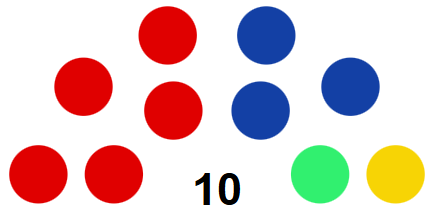
\includegraphics[width = 0.7\textwidth]{LaTeX/task3/img/Screenshot 2026-05-22 024410.png}}

    Рисунок 2. Распределение методом Д'Ондта. Шакально конечно, но картинки на Википедии нет, пришлось делать самому, а .svg латех не поддерживает
\end{center}

\begin{center}
    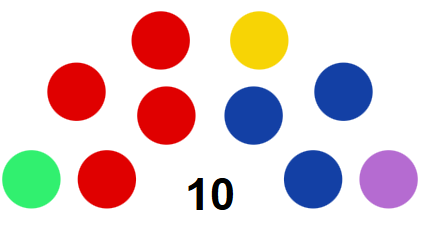
\includegraphics[width = 0.7\textwidth]{LaTeX/task3/img/Screenshot 2026-05-22 025556.png}

    Рисунок 3. Распределение методом Сент-Лагю
\end{center}
Как видно из таблицы 3.1 метод Д'Ондта завысил результаты лидирующей партии, а партии E вообще не досталось мест, в то время как метод Сент-Лагю более близок к точному кол-ву <<заслуженных>> мест.